\scanpage{20}nier (ou, ce qui revient au même, $c$) est bien déterminée. Les unipotents qui définissent ladite filtration, en termes d'un $i$ qui la définit, sont
% Typed interlinear insertion; the connected handwritten curve has no arrowhead.
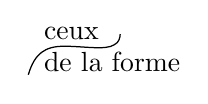
\begin{tikzpicture}[baseline=(base.base),x=1em,y=1em]
  \node[anchor=base west,inner sep=0] (base) at (0,0) {de la forme};
  \node[anchor=base west,inner sep=0] at (0,1.15) {\inserted{ceux}};
  \draw[line width=.45pt] (-.55,-.12) .. controls (-.32,.65) and (.05,.91) .. (.75,.91)
    .. controls (1.45,.91) and (2.25,.76) .. (2.55,.96)
    .. controls (2.73,1.04) and (2.77,1.23) .. (2.77,1.35);
\end{tikzpicture}
$\exp(e)$, où $e$ parcourt $\handwritten{\unsure{\mathfrak{g}|\mathscr{G}}}(2)^{\handwritten{*}}+\operatorname{Fil}^{\handwritten{3}}(\handwritten{\mathfrak{g}})$. Ils forment une classe de conjugaison d'éléments de $U$ \uline{par} $P$ (NB mais pas par $U$), les classes de conjugaison \uline{par} $U$ s'identifiant aux ensembles de la forme $(\exp(e)\handwritten{\mid}e\handwritten{\in}a+\operatorname{Fil}^{\handwritten{3}}(\handwritten{\mathfrak{g}}\unsure{.|,}))$, où $a\handwritten{\in\mathfrak{g}}(2)^{\handwritten{*}}$ est un élément quelconque.\deleted{d\unsure{e}}

\uline{Cas principal}. Pour qu'on ait\hspace{1.5em}$(1)=0$, il faut et suffit que \deleted{l'homomor} la classe d'homomorphismes $f:\operatorname{Sl}(2,k)\hspace{1.5em}G$ envisagée soit ``princi\unsure{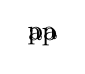
\begin{tikzpicture}[baseline=(pa.base),x=1em,y=1em]
  \node[anchor=base west,inner sep=0] (pa) at (0,0) {pa};
  \node[anchor=base west,inner sep=0] at (.015,-.02) {ap};
\end{tikzpicture}}le'' au sens de Dynkin-Kostant. Alors le parabolique associé $P$ est un Borel
% Slanted left-margin note. Its five source lines and the separate underlined ex are retained.
\reversemarginpar
\margin{\handwritten{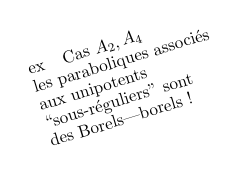
\begin{tikzpicture}[x=1em,y=1em,rotate=17,scale=.62,transform shape]
  \node[anchor=base west,inner sep=0] at (0,4.4) {\uline{ex}};
  \node[anchor=base west,inner sep=0] at (2.1,4.4) {Cas $A_2,A_4$};
  \node[anchor=base west,inner sep=0] at (0,3.3) {les paraboliques associés};
  \node[anchor=base west,inner sep=0] at (0,2.2) {aux unipotents};
  \node[anchor=base west,inner sep=0] at (0,1.1) {``sous-réguliers'' sont};
  \node[anchor=base west,inner sep=0] at (0,0) {des \unsure{Borels|borels} !};
\end{tikzpicture}}}
\normalmarginpar
(la réciproque n'étant pas vraie \deleted{sans doute}, cf table de Dynkin), et le groupe $Z_o$ est le groupe unité (i.e. $\operatorname{Dyn}_c$ est un torseur sous $G$),
% The first cell has an l-like stem and two curved companion traces. Their alphabet and chronological order are unresolved.
\unsure{
\begin{tikzpicture}[baseline=(l.base),x=1em,y=1em]
  \node[anchor=base west,inner sep=0] (l) at (0,0) {l};
  \draw[line width=.4pt] (.34,.59) .. controls (.04,.79) and (-.02,.42) .. (.18,.35)
    .. controls (.42,.26) and (.39,.02) .. (.08,.04);
  \draw[line width=.3pt] (.19,-.08) -- (.19,.69);
\end{tikzpicture}a} réciproque n'étant pas vraie sans doute.
% archive sheet number: 19
